% The worked example of Sec. 3.3: one entry, two access paths, and the state
% that a pseudo-transaction removes.
%
% Drawn in TikZ (not an imported image) so the figure ships as source in the
% arXiv submission and needs no external toolchain to rebuild.
%
% The picture must make exactly one thing obvious: publishing into the index
% and into the recency list with two stores leaves a MIDDLE state in which a
% reader finds E by key and finds it in no position, and one commit has no
% middle state at all. The absent column is the whole argument; everything
% else in the drawing is scaffolding for it.
%
% ANCHORED, not a float, for the reason documented at tab:fssense: this figure
% belongs beside the prose that sets it up, and as a float it would read
% correctly only by the accident of landing on the same page.
\par\medskip\noindent\begin{minipage}{\linewidth}
\centering
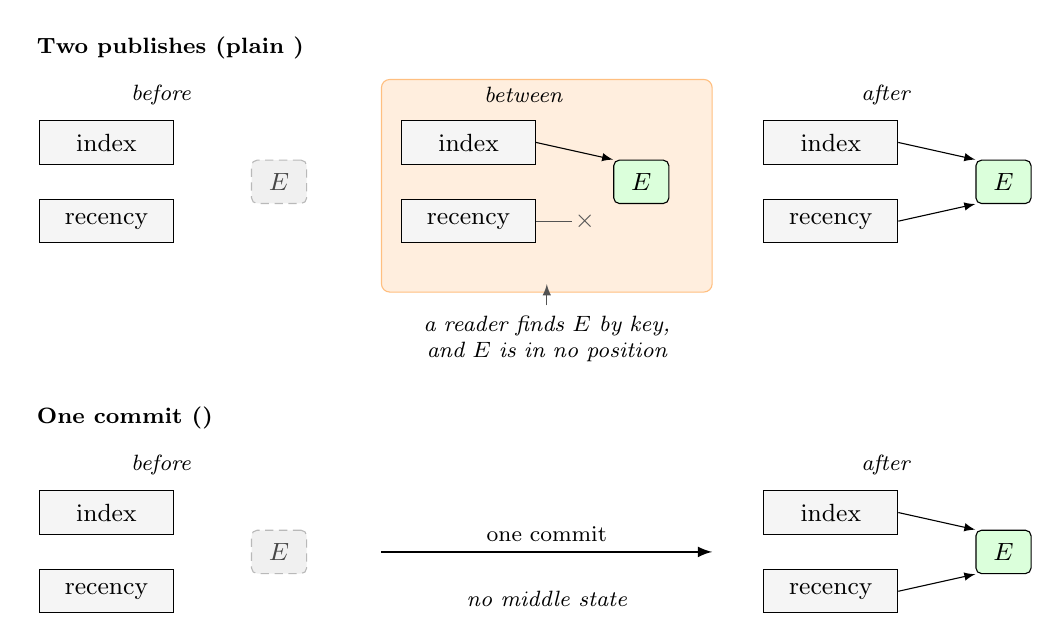
\begin{tikzpicture}[
  font=\small,
  box/.style   = {draw, minimum width=17mm, minimum height=5.5mm, fill=gray!8,
                  anchor=west, font=\small},
  ent/.style   = {draw, rounded corners=2pt, minimum width=7mm,
                  minimum height=5.5mm, fill=green!14},
  gone/.style  = {draw, rounded corners=2pt, minimum width=7mm,
                  minimum height=5.5mm, fill=gray!12, draw=gray!55,
                  text=gray!55!black, densely dashed},
  arr/.style   = {-latex, thin},
  stub/.style  = {thin, gray!65!black},
  hdr/.style   = {font=\footnotesize\bfseries},
  note/.style  = {font=\footnotesize\itshape, align=center},
  skew/.style  = {fill=orange!13, draw=orange!50, rounded corners=3pt},
]

% ===== row 1: two publishes ==============================================
% highlight behind the middle column, drawn first so it sits underneath
\fill[skew] (4.35,-0.55) rectangle (8.55,2.15);

\node[hdr, anchor=west] at (-0.15,2.55) {Two publishes (plain \rcu)};

% ---- column 1: before ---------------------------------------------------
\node[note] at (1.55,1.95) {before};
\node[box] (i1) at (0,1.35) {\code{index}};
\node[box] (r1) at (0,0.35) {\code{recency}};
\node[gone] (e1) at (3.05,0.85) {$E$};

% ---- column 2: between (the skew) ---------------------------------------
\node[note] at (6.15,1.95) {between};
\node[box] (i2) at (4.6,1.35) {\code{index}};
\node[box] (r2) at (4.6,0.35) {\code{recency}};
\node[ent]  (e2) at (7.65,0.85) {$E$};
\draw[arr] (i2.east) -- (e2.north west);
\draw[stub] (r2.east) -- ++(0.45,0) node[right, inner sep=1pt] {$\times$};

% ---- column 3: after ----------------------------------------------------
\node[note] at (10.75,1.95) {after};
\node[box] (i3) at (9.2,1.35) {\code{index}};
\node[box] (r3) at (9.2,0.35) {\code{recency}};
\node[ent]  (e3) at (12.25,0.85) {$E$};
\draw[arr] (i3.east) -- (e3.north west);
\draw[arr] (r3.east) -- (e3.south west);

\node[note, text width=42mm] at (6.45,-1.15)
  {a reader finds $E$ by key,\\ and $E$ is in no position};
\draw[stub, -latex] (6.45,-0.72) -- (6.45,-0.45);

% ===== row 2: one commit =================================================
\node[hdr, anchor=west] at (-0.15,-2.15) {One commit (\pseudotxn)};

\node[note] at (1.55,-2.75) {before};
\node[box] (i4) at (0,-3.35) {\code{index}};
\node[box] (r4) at (0,-4.35) {\code{recency}};
\node[gone] (e4) at (3.05,-3.85) {$E$};

\node[note] at (10.75,-2.75) {after};
\node[box] (i5) at (9.2,-3.35) {\code{index}};
\node[box] (r5) at (9.2,-4.35) {\code{recency}};
\node[ent]  (e5) at (12.25,-3.85) {$E$};
\draw[arr] (i5.east) -- (e5.north west);
\draw[arr] (r5.east) -- (e5.south west);

\draw[-latex, thick] (4.35,-3.85) -- (8.55,-3.85)
  node[midway, above, font=\footnotesize] {one commit};
\node[note] at (6.45,-4.45) {no middle state};

\end{tikzpicture}
\captionof{figure}{Inserting entry $E$ into a cache with two access paths;
dashed $E$ is built but not yet reachable. With
two publications the order is a choice and neither choice is right: publishing
into the index first leaves the shaded state, in which a lookup finds $E$ and
the recency list does not contain it (publishing into the list first leaves the
mirror image). The window is not a few instructions --- the writer can be
preempted inside it. One commit names both slots in a single record set, so the
shaded state does not exist.}
\label{fig:skew}
\end{minipage}\par\medskip
